%!TEX root = ../slopecd.tex
\section{Theory}\label{sec:theory}
%%%%%%%%%%%%%%%%%%%%%%%%%%%%%%%%%%%%
\subsection{Directional Derivatives}%
\label{sec:directional-derivatives}
%%%%%%%%%%%%%%%%%%%%%%%%%%%%%%%%%%%%

\subsubsection{The Sorted \texorpdfstring{\(\ell_1\)}{l1}
  Norm}

\begin{theorem}
  \label{thm:sl1-directional-derivative} Let \(h_0 \in \big(0, \min_{i,j \in
    \{i \mid \beta_i \neq 0\}}\big| |\beta_i| - |\beta_j| \big|/\max_k|v_k| \big]\) and
  define \(\sigma\) to be the permutation such that
  \[
    |\beta + h_0v|_{\sigma(1)} \geq |\beta + h_0v |_{\sigma(2)}
    \geq \cdots \geq |\beta + h_0v|_{\sigma(p)}.
  \]
  The directional derivative for the sorted \(\ell_1\) norm, \(J(\beta)\), is
  \[
    D_v J(\beta) =
    \sum_i \sum_{j \in \mathcal{B}_i} \lambda_j v_{\sigma(j)}\sign(\beta_{\sigma(j)} + h_0v_{\sigma(j)})\]
  where
  \[
    \mathcal{B}_i = \{j \mid |\beta_j| = c_i\},\qquad
    c_1 > c_2 > \cdots > c_m \geq 0,
  \]
  such that \(m\) is the number of clusters.
  \jl{We need something that doesn't define clusters multiple times.}
  \mathurin{Good remark, I guess we could avoid naming the variable \(i\) since above we have \(i\) and \(j\) being both in \([p]\) while here \(i\) would in fact be in \([n_{clusters}/n_{groups}]\). \(g\) for groups, as used in group Lasso? "For a fixed \(\beta\), let \(G\) be the number of different values taken by \(\abs{\beta_j}\), i.e. the number of groups, and let \((\cB_g)_{g \in G}\) be a partition of \([p]\) such that \(\forall (j, j') \in \cB_g, \abs{\beta_j} = \abs{\beta_{j'}}\)}
  \jl{Thanks, yes that would work.
    I have tried something slightly different
    here, however, which may be enough for us.
  }

\end{theorem}
\begin{proof}
  The directional derivative for the sorted \(\ell_1\) norm and a direction
  \(v\) with \(\lVert v \rVert = 1\) is
  \begin{equation}
    \label{eq:sl1-directional-derivative}
    \begin{aligned}
      D_v J(\beta) & = \lim_{h \searrow 0} \frac{J(\beta + h v) - J(\beta)}{h}                                                                    \\
                   & = \lim_{h \searrow 0} \frac{\sum_{j=1}^p\lambda_j\big(|\beta + vh|_{\sigma(j)} - |\beta|_{(j)}\big)}{h}                      \\
                   & = \lim_{h \searrow 0}\frac{\sum_i \sum_{j \in \mathcal{B}_i} \lambda_j\big(|\beta + vh|_{\sigma(j)} - |\beta|_{(j)}\big)}{h} \\
    \end{aligned}
  \end{equation}
  Assume without loss of generality that \(c_m = 0\).
  Then
  \[
    \sum_{j \in \mathcal{B}_m}\frac{\lambda_j \big( |\beta + vh|_{\sigma(j)} - |\beta|_{(j)}\big)}{h}
    = \sum_{j \in \mathcal{B}_m} \lambda_j \sign(\beta + hv)_{\sigma(j)}v_{\sigma(j)}.
  \]
  Next, recall the construction of \(h_0\) and
  observe that \(\sign(\beta_j + hv_j) = \sign(\beta_j)\)
  and \(\sigma(j) = (j)\) for all \(j \notin \mathcal{B}_m\)
  whenever \(0 < h < h_0\).
  It follows that
  \[
    \sum_{j \in \mathcal{B}_i} \frac{\lambda_j\big(|\beta + hv|_{\sigma(j)} - |\beta|_{(j)}\big)}{h}
    = \sum_{j \in \mathcal{B}_i} \lambda_j\sign(\beta + vh)_{\sigma(j)}v_{\sigma(j)}.
  \]
  From this, we see that \eqref{eq:sl1-directional-derivative} reduces to
  \[
    \lim_{h \searrow 0} \sum_i \sum_{j \in \mathcal{B}_i} \lambda_j\sign(\beta + vh)_{\sigma(j)}v_{\sigma(j)}
    = \sum_i \sum_{j \in \mathcal{B}_i} \lambda_j\sign(\beta + vh_0)_{\sigma(j)}v_{\sigma(j)}.
  \]
\end{proof}

\begin{remark}
  Using \cref{thm:sl1-directional-derivative}, we see that
  the directional derivative for \eqref{eq:slope-problem} is
  \[
    D_v P(\beta) = v^T \big(\nabla L(\beta)\big) + D_v J(\beta).
  \]
\end{remark}

\subsection{Coordinate Updates}%
\label{sec:coordinate-updates}

Assume that we want to compute the coordinate update for the \(q\)th cluster
\(\mathcal{C}_q\) under the constraint that \(\sign(\beta) = s\) and
\(|\beta_j| = |\tilde \beta|\) for all \(j \in \mathcal{C}_q\).
To avoid verbosity, let
\(u = c_q\).
We have
\[
  \begin{aligned}
    P(\beta) & =  \frac{1}{2} \lVert y - X\beta\rVert_2^2 + J(\beta)                                                                                                                                                                                                                                   \\
             & = \frac{1}{2} \lVert y - X_{\bar{\mathcal{C}_q}} \beta_{\bar{\mathcal{C}_q}} - \big(X_{\mathcal{C}_q} s_{\mathcal{C}_q}\big)\tilde\beta  \rVert_2^2 + \sum_{k \notin {\mathcal{C}_q}} \lambda_{(k)^-}|\beta_k| + \bigg(\sum_{k \in {\mathcal{C}_q}} \lambda_{(k)^-}\bigg)|\tilde\beta|.
  \end{aligned}
\]
Now let \(\tilde y = X_{\bar{\mathcal{C}_q}} \beta_{\bar{\mathcal{C}_q}}\)
such that \(y - \tilde y\) is the \emph{partial residual} and take the
derivate with respect to \(\tilde\beta\), yielding
\begin{equation}
  \label{eq:cluster-grad}
  \partial_{\tilde\beta}
  P(\beta) = (\tilde y - y)^T X_{\mathcal{C}_q} s_{\mathcal{C}_q} + s_{\mathcal{C}_q}^T X_{{\mathcal{C}_q}}^T X_{\mathcal{C}_q} s_{\mathcal{C}_q} \tilde\beta + \partial_{\tilde\beta}\Bigg(\bigg(\sum_{k \in {\mathcal{C}_q}} \lambda_{(k)^-}\bigg)|\tilde\beta| + \sum_{k \notin \mathcal{C}_q}\lambda_{(k)^-}|\beta_k|\Bigg),
\end{equation}
where the last term is the partial subdifferential of the sorted \(\ell_1\)
norm. The optimality condition for this sub-problem is \( \partial_{\tilde
\beta} P(\beta) \in \boldsymbol{0}. \)

\begin{theorem}
  \label{thm:cluster-subdifferential}
  The partial subdifferential for the sorted \(\ell_1\) norm with respect
  to \(\tilde\beta\) is
  \[
    \partial =
    \begin{cases}
      \{\sign(\tilde\beta) S\big(C(\tilde\beta)\big)\}                    & \text{if } \tilde\beta \neq c_i \neq 0, \\
      [-S(\mathcal{C}_m), S(\mathcal{C}_m)]                               & \text{if } \tilde\beta = 0,             \\
      [\sign(\tilde\beta)S\big( C(c_i - \sign(\tilde\beta)\varepsilon_i)\big), \sign(\tilde\beta)S\big(C(c_i + \sign(\tilde\beta)\varepsilon_i)\big)] & \text{if } |\tilde\beta| = c_i,
    \end{cases}
  \]
  where \(\varepsilon \in (0, \min_{j}|c_i - c_j|)\).
\end{theorem}
\begin{proof}
  Let \(f(\tilde\beta) = |\tilde\beta|\sum_{k \in \mathcal{C}_q}\lambda_{(k)^-} + \sum_{k \notin \mathcal{C}_q} \lambda_{(k)^-}|\beta_k|\).
  \(g\) is a subgradient of \(f\) at \(x\) if
  \begin{equation}
    \label{eq:subgrad-ineq}
    |y|\sum_{j \in C(y)}\lambda_{(j)^-} + \sum_{j \notin C(y)}\lambda_{(j)^-}|\beta_j| 
    \geq |x|\sum_{j \in C(x)} \lambda_{(j)^-} + \sum_{j \notin C(x)}\lambda_{(j)^-}|\beta_j| + g(y - x).
  \end{equation}
  Without loss of generality, since \(f\) is convex, assume that we have
  a vector \(\beta\) such that there are two clusters: one corresponding
  to \(\tilde\beta\), which we are optimizing over, and
  one additional cluster \(\mathcal{C}_q\) with corresponding
  coefficient \(c_q\). Then we can rewrite \eqref{eq:subgrad-ineq} as
  \[
    |y|S\big(C(y)\big) + c_q S\big(\widebar{C(y)}\big) \geq
    |x| S\big(C(x)\big) + c_q S\big(\widebar{C(x)}\big) + g(y - x).
  \]
  First observe that any \(g\) is permissible whenever \(x = y\).

  At \(x = 0\), \eqref{eq:subgrad-ineq} reduces to
  \[
    |y|S\big(C(y)\big) + c_q S\big(\widebar{C(y)}\big)
    \geq c_q(\mathcal{C}_1) + gy.
  \]
  Because \(f\) is convex, it is sufficient to consider \(|y| < c_q\).
  In this case, we get
  \[
    |y|S(\mathcal{C}_2) \geq gy,
  \]
  which means that \(-S(\mathcal{C}_2) \leq g \leq S(\mathcal{C}_2)\).

  If \(x = c_q\), \eqref{eq:subgrad-ineq} becomes
  \[
    |y|S\big(C(y)\big) + x S\big(C(x)\big) \geq x(S(\mathcal{C}_1) + S(\mathcal{C}_2)) + g(y - x).
  \]
  Then, for \(y > x\), we have
  \[
    y\big(S(\mathcal{C}_1) - g\big) + x\big(g - S(\mathcal{C}_1)\big) \geq 0,
  \]
  which means that \(g \leq S(\mathcal{C}_1)\).
  Then, for \(0 < y < x\), we see
  \[
    y\big(S(\mathcal{C}_2) - g\big) + x(g - S(\mathcal{C}_2)\big) \geq 0,
  \]
  and hence \(g \geq S(\mathcal{C}_2)\).
  Using the same argument for \(x = -c_q\), we find that we in this case
  must have \(g\) such that 
  \(-S(\mathcal{C}_1) \geq g \geq - S(\mathcal{C}_2)\).
  For all other choices of \(x\), \(f\) is differentiable with
  derivative \(\sign(\tilde\beta)S\big(C(\tilde\beta)\big)\).
\end{proof}

The objective and subgradient for the cluster-wise problem are shown in
\cref{fig:cluster-grad-obj}.

\begin{figure}[htbp]
  \centering
  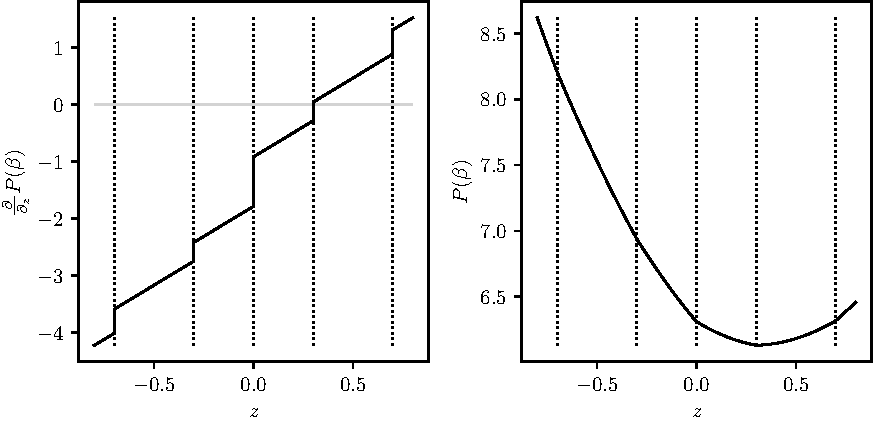
\includegraphics[]{figures/clusterupdate-grad-obj}
  \caption{%
    Objective and gradient under the constraint that we have a fixed
    cluster.
    The optimum is found at \(\tilde\beta = 0.3\).
  }%
  \label{fig:cluster-grad-obj}
\end{figure}

